\documentclass[12pt]{article}

\usepackage{geometry}
\usepackage{polski}
\usepackage{amsthm}
\usepackage{amsfonts}
\usepackage{graphicx}
\usepackage{float}
\usepackage{mathtools}

\theoremstyle{twierdzenie}
\newtheorem{theorem}{Twierdzenie}[section]

\theoremstyle{definition}
\newtheorem{defi}{Definicja}[section]
\begin{document}
\begin{center}
\begin{Large}
\textbf{Matematyka Ubezpieczeń Majątkowych i Osobowych}\\
\end{Large}
\begin{large}
Piotr Bocian
\end{large}

\end{center}
\tableofcontents
\section{Wprowadzenie}
Niniejszy dokument zawiera w sobie obie części projektu realizowanego na przedmiot Matematyka Ubezpieczeń Majątkowych i Osobowych. Część pierwsza (rozdziały $2-5$) przedstawia zagadnienia dotyczące obliczenia rozkładów portfeli złożonych oraz ich aproksymacji standardowymi rozkładami. W części drugiej (rozdziały $6-8$) zajmujemy się analizą portfeli ze względu na miary ryzyka oraz obliczaniem prawdopodobieństwa ruiny.

\section{Rozkłady portfeli} 
Niech $X_i$, $i\geq 1$ będą szkodami o rozkładzie binomialnym $b(k,10,1/2)$.\\
Definiujemy portfele
$$S_N=X_1+\dots+X_N,$$
$$S_M=X_1+\dots+X_M,$$
$$S_K=X_1+\dots+X_K,$$
gdzie $N\sim b(k,n,p)$, $M\sim Poi(\lambda)$, $K\sim Geo(p)$. Dodatkowo $N,M,K$ mają wartość średnią równą $30$. Dla poszczególnych rozkładów mamy:
$$\mathbb{E}N=np,$$
$$\mathbb{E}M=\lambda,$$
$$\mathbb{E}K=\frac{1}{p-1}.$$
Możemy więc przyjąć, że $N\sim b(k,60,1/2)$ oraz $M\sim Poi(30)$ i $K\sim Geo(1/31)$
\subsection{Metoda funkcji tworzących}
Funkcja tworząca rozkładu binomialnego $b(k,10,1/2)$ ma postać
$$P_{X_i}(t)=\sum_{k=0}^{10}{10\choose k}\left(\frac{1}{2}\right)^k\left(\frac{1}{2}\right)^{10-k}t^k=\left(\frac{1}{2}+\frac{1}{2}t\right)^{10}$$
\subsubsection{Portfel $S_N$}
Zmienna $N$ ma rozkład binomialny $b(k,60,1/2)$. Stąd funkcja tworząca jest dana jako
$$P_N(t)=\sum_{k=0}^{60}{60\choose k}\left(\frac{1}{2}\right)^k\left(\frac{1}{2}\right)^{60-k}t^k=\left(\frac{1}{2}+\frac{1}{2}t\right)^{60}$$
Stąd otrzymujemy funkcję tworzącą $S_N$ daną jako
$$P_{S_N}(t)=P_N(P_{X_i}(t))=\left(\frac{1}{2}+\frac{1}{2}\left(\frac{1}{2}+\frac{1}{2}t\right)^{10}\right)^{60}$$
\subsubsection{Portfel $S_M$}
Zmienna $M$ ma rozkład Poissona $Poi(30)$. Wynika z tego, że funkcja tworząca $M$ jest postaci
$$P_M(t)=\sum_{k=0}^\infty \frac{e^{-30}{30^k}}{k!}t^k=e^{30t-30}$$
Stąd funkcja tworząca $S_2M$ jest dana jako
$$P_{S_M}(t)=P_M(P_{X_i}(t))=\exp\left(30\left(\frac{1}{2}+\frac{1}{2}t\right)^{10}-30\right)$$
\subsubsection{Portfel $S_K$}
Zmienna $K$ ma rozkład geometryczny $Geo(1/31)$. Funkcja tworząca jest dana jako:
$$P_K(t)=\sum_{k=0}^\infty\left(\frac{30}{31}\right)^k\frac{1}{31}t^k=\frac{1/31}{1-\frac{30}{31}t}$$
Funkcja tworząca $S_K$ jest więc dana jako
$$P_{S_K}(t)=P_K(P_{X_i}(t))=\frac{1}{31}\left(1-\frac{30}{31}\left(\frac{1}{2}+\frac{1}{2}t\right)^{10}\right)^{-1}$$
\subsection{Wykresy rozkładów}
\begin{figure}[h]
\begin{center}
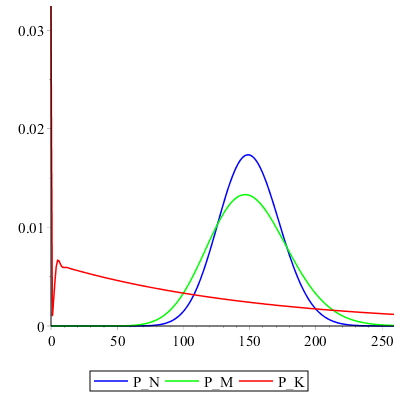
\includegraphics[scale=.8]{wykres}
\caption{Wykresy rozkładów portfeli wyliczonych za pomocą metody funkcji tworzących.}
\end{center}


\end{figure}
\subsection{Parametry rozkładów portfeli}
W tej części przyjrzymy się trzem parametrom rozkładów portfeli $S_N,S_M,S_K$. Przypomnijmy, że wariancja rozkładu $S_i$ jest określona jako 
$$VarS_i=\mathbb{E}S_i^2-(\mathbb{E}S_i)^2$$
Do wyliczenia wartości oczekiwanej będzie nam potrzebna funkcja tworząca momenty
$$M_{S_i}(t)=P_{S_i}(e^t)$$
Wtedy wartości oczekiwane poszczególnych momentów są dane przez
$$\mathbb{E}S_i=M_{S_i}'(0),\ \mathbb{E}S_i^2=M_{S_i}''(0)$$
Wartości powyższych parametrów rozkładów portfeli $S_N,S_M,S_K$ zostały zawarte w poniższej tabeli
\begin{center}
$$
\begin{tabular}{ |c|c|c|c| } 
 \hline
& \multicolumn{3}{|c|}{Portfel} \\
\hline
Parametr & $S_N$ & $S_M$ & $S_K$ \\
\hline

$\mathbb{E}S_i$ & 150 & 150 & 150\\ 
$\mathbb{E}S_i^2$  & 22950 & 23325 & 45825 \\ 
$VarS_i$ & 450  & 825 & 23325\\
\hline
\end{tabular}
$$
\end{center}
Jak widać zachodzi nierówność 
$$VarS_N<VarS_M<VarS_K.$$
\section{Histogramy}
Z rozkładów portfeli wygenerowano próby wielkości 50. Poniżej znajdują się histogramy prób wraz z wykresem gęstości. 
\begin{figure}[H]
\begin{center}
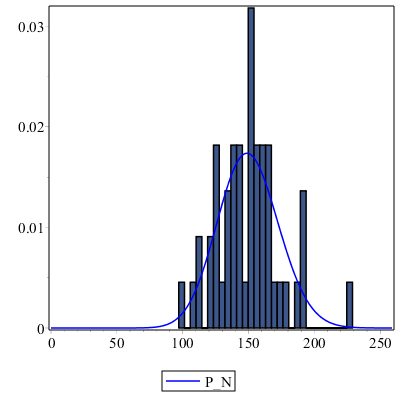
\includegraphics[scale=.5]{histN}
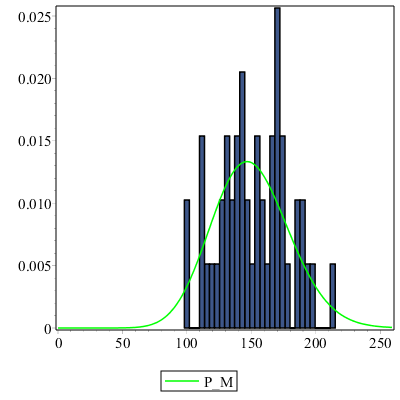
\includegraphics[scale=.5]{histM}
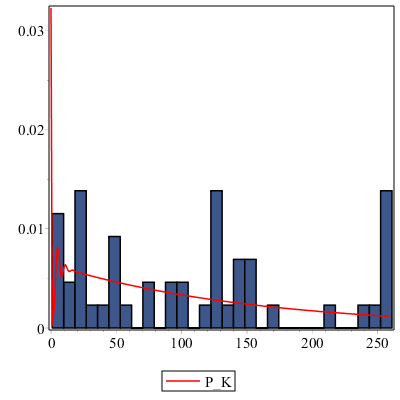
\includegraphics[scale=.5]{histK}
\end{center}

\end{figure}
W przypadku wszystkich wykresów widzimy, że histogram 50 wartości daje słabo widoczne przybliżenie rozkładu.
\section{Przybliżanie rozkładem normalnym}
\subsection{Obliczanie parametrów}
Funkcja gęstości rozkładu normalnego jest dana przez
$$\Phi(\mu,\sigma)=\frac{1}{\sigma\sqrt{2\pi}}e^{\frac{-(x-\mu)^2}{2\sigma^2}}$$
W celu przybliżenia rozkładu $S_i$ rozkładem normalnym obliczamy parametry
$$\mu=\mathbb{E}S_i,\ \sigma=\sqrt{VarS_i}$$
\begin{center}
$$
\begin{tabular}{ |c|c|c|c| } 
 \hline
& \multicolumn{3}{|c|}{Portfel} \\
\hline
Parametr & $S_N$ & $S_M$ & $S_K$ \\
\hline

$\mu$ & 150 & 150 & 150\\ 
$\sigma$ &  21.2132 & 28.72281 & 152.7252 \\ 

\hline
\end{tabular}
$$

\end{center}
\newpage
\subsection{Wykresy}
Poniższe wykresy przedstawiają wykresy rozkładów portfeli wraz z ich przybliżeniami rozkładem normalnym.
\begin{figure}[H]
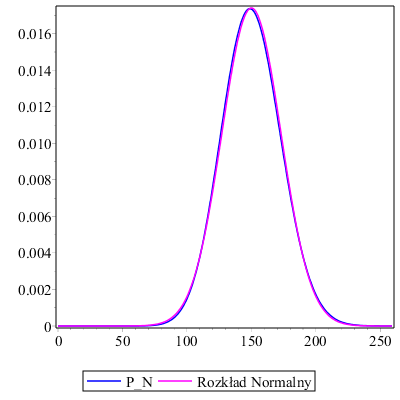
\includegraphics[scale=.5]{normalnydlaN}
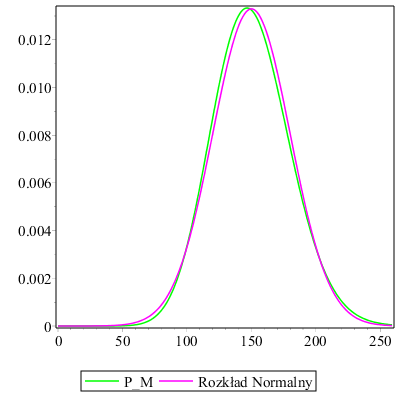
\includegraphics[scale=.5]{normalnydlaM}
\begin{center}
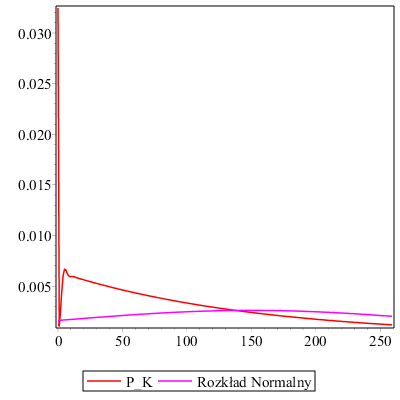
\includegraphics[scale=.5]{normalnydlaK}
\end{center}

\end{figure}
\section{Przybliżanie rozkładem gamma}
\subsection{Obliczanie parametrów}
Funkcja gęstości rozkładu gamma jest dana przez
$$g(x,\alpha,\beta)=\frac{\beta^\alpha}{\Gamma(\alpha)}x^{\alpha-1}e^{-\beta x}$$
W celu przybliżenia rozkładu $S_i$ rozkładem gamma obliczamy parametry $\alpha,\beta$ określone jako
$$\mathbb{E}[S_i]=\frac{\alpha}{\beta},\ Var[S_i]=\frac{\alpha}{\beta^2}$$

\begin{center}
$$
\begin{tabular}{ |c|c|c|c| } 
 \hline
& \multicolumn{3}{|c|}{Portfel} \\
\hline
Parametr & $S_N$ & $S_M$ & $S_K$ \\
\hline

$\alpha$ & 300/7 & 25 & 25/26 \\ 
$\beta$ & 2/7 & 1/6 & 1/156 \\ 

\hline
\end{tabular}
$$

\end{center}
\newpage
\subsection{Wykresy}
Poniższe wykresy przedstawiają wykresy rozkładów portfeli wraz z ich przybliżeniami rozkładem gamma.
\begin{figure}[H]
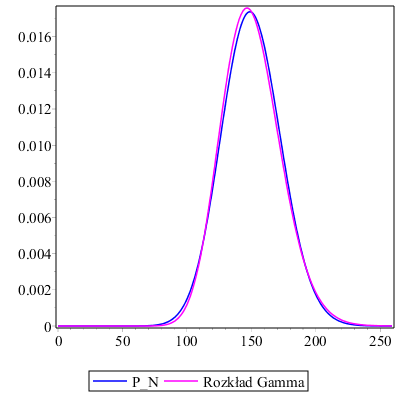
\includegraphics[scale=.5]{gammadlaN}
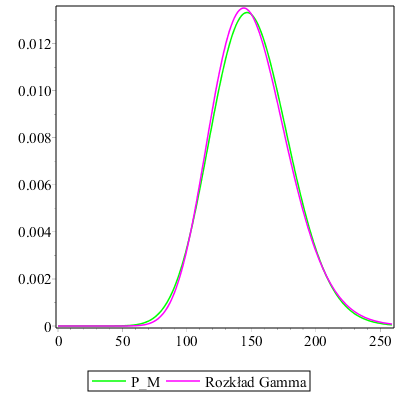
\includegraphics[scale=.5]{gammadlaM}
\begin{center}
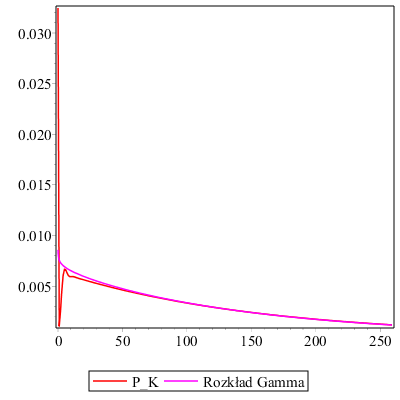
\includegraphics[scale=.5]{gammadlaK}
\end{center}
\end{figure}
\section{Uporządkowanie portfeli}
Dla dwóch zmiennych losowych $X,Y$ wprowadzamy następującą relację porządku:
$$X<_{CX}Y\Leftrightarrow (\forall d\in\mathbb{R})\left(\mathbb{E}\left[(X-d)_+\right]\leq \mathbb{E}\left[(Y-d)_+\right]\right)$$
Mając tak zdefiniowaną relację, w tej części zbadamy uporządkowanie zmiennych $S_N$, $S_M$ i $S_K$. W tym celu wykorzystamy metodę zwaną kryterium Karlina-Novikowa.

\begin{theorem}[Kryterium Karlina-Novikowa]
Jeżeli zmienne losowe $X,Y$ spełniają $\mathbb{E}[X]\leq\mathbb{E}[Y]$ oraz istnieje $x_0$, takie że:
\begin{itemize}
\item $(\forall x<x_0)(F_Y(x)\geq F_X(x))$
\item $(\forall x>x_0)(F_Y(x)\leq F_X(x))$,
\end{itemize}
to $X<_{CX}Y$.
\end{theorem}
W naszym przypadku, wartości oczekiwane rozkładów portfeli są równe. Dodatkowo, na poniższych wykresach przedstawione zostały dystrybuanty rozkładów portfeli $S_N,S_M,S_K$. 
\begin{figure}[H]
\begin{center}
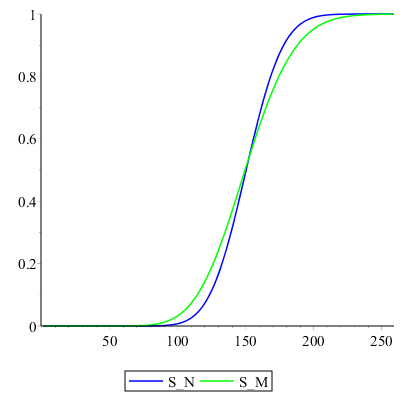
\includegraphics[scale=.5]{cdfPNPM}
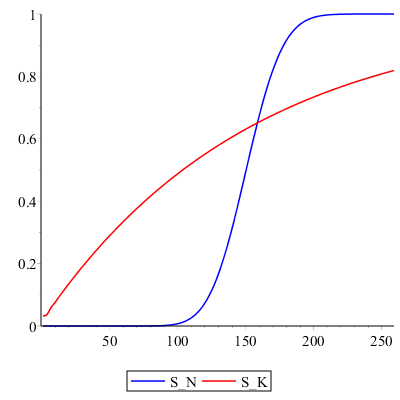
\includegraphics[scale=.5]{cdfPNPK}
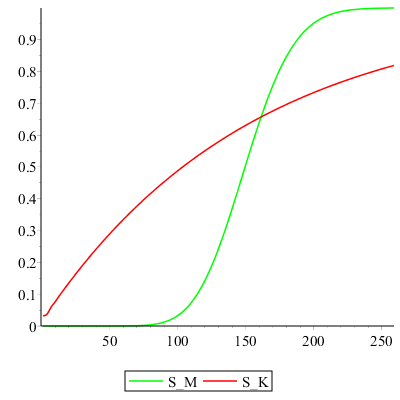
\includegraphics[scale=.5]{cdfPMPK}
\end{center}
\end{figure}

Jak widać, korzystając z kryterium Karlina-Novikowa otrzymujemy następujące zależności:
$$S_N<_{CX} S_M,\ S_N<_{CX} S_K,\ S_M<_{CX} S_K$$
\newpage
\section{Miary ryzyka portfeli}
W tym rozdziale przyjrzymy się rozkładom portfeli w kontekście miar ryzyka. Na początku przypomnimy miary potrzebne w kontekście naszego zagadnienia.
\begin{defi}
Dla zmiennej losowej $X$ i $p\in(0,1)$ definiujemy następujące miary ryzyka:
\begin{enumerate}
\item \textit{Value at Risk}:
$$VaR_X(p)=\inf\lbrace t:F_X(t)\geq p\rbrace.$$
\item \textit{Expected Shortfall}:
$$ES_X(p)=\mathbb{E}[(X-VaR_X(p))_+]$$
\item \textit{Tail Value at Risk}:
$$TVaR_X(p)=\frac{1}{1-p}\int_p^1 VaR_X(u)du,$$
lub
$$TVaR_X(p)=VaR_X(p)-\frac{ES_X(p)}{1-p}$$
\end{enumerate}
\end{defi}
Z uwagi na to, że zmienne które rozpatrujemy są dyskretne, użyjemy drugiego wzoru na obliczenie $TVaR$.
\subsection{Wykres $TVaR$}
Poniższy wykres przedstawia wartość miary $TVaR$ dla naszych portfeli $S_N,S_M,S_K$. 
\begin{figure}[H]
\begin{center}
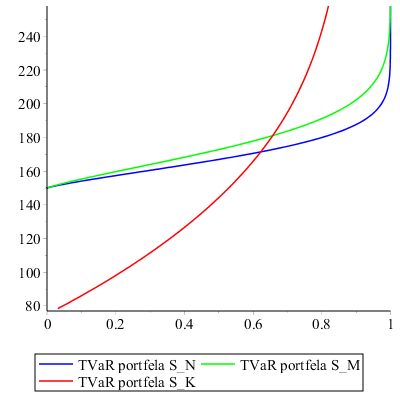
\includegraphics[scale=.7]{tvar2}
\end{center}
\end{figure}
Jak widać na wykresie najmniejszym ryzykiem cechuje się $S_K$ - największym zaś $S_M$.
\newpage
\section{Prawdopodobieństwo ruiny}
Niech $R_n=u+160n-(W_1+\dots+W_n)$, gdzie $W_i$ są niezależne. Chcemy wyliczyć przybliżenia prawdopodobieństwa ruiny w przypadkach gdy $W_i$ mają kolejno rozkłady takie jak $S_N,S_M,S_K$.\\
Ciąg $R_n$ możemy zapisać jako błądzenie losowe startujące z poziomu $u$:
$$R_n=u+(c-W_1)+\dots+(c-W_n).$$
Wtedy prawdopodobieństwo ruiny, jest określone jako
$$\psi(u)=P\left(\bigcup_{i\geq 1}\lbrace R_i<0\rbrace\right)=P\left(\bigcup_{i\geq 1}\lbrace S_i-ci>u\rbrace\right)=P\left(\max (S_i-ci:\ i\geq 1)>u\right)$$
W naszym przypadku $c=160$ więc możemy napisać:
$$R_n=u+(160-W_1)+\dots+(160-W_n).$$
\subsection{Współczynnik dopasowania}
Dla zmiennych losowych $(W_i)_{i\geq 1}$ mających ten sam rozkład i $\mathbb{E}[W]<c$, współczynnik dopasowania definiujemy jako dodatnie rozwiązanie równania 
$$\exp(-cr)M_w(r)=1,$$
gdzie $M_W(t)$ jest funkcją tworzącą momenty zmiennych $W_i$. Współczynnik dopasowania oznaczamy przez $R(W,c)$.\\
Obliczymy teraz współczynniki dopasowania w naszych trzech przypadach. 
Przypomnijmy najpierw parametry naszych rozkładów:
\begin{center}
$$
\begin{tabular}{ |c|c|c|c|c| } 
 \hline
& \multicolumn{4}{|c|}{Zmienna} \\
\hline
Parametr & $N$ & $M$ & $K$ & $X$ \\
\hline

\text{Wartość oczekiwana} & 30 & 30 & 30 & 5 \\ 
\text{Wariancja} & 15  & 30 & 930 & 2.5 \\
\hline
\end{tabular}
$$
\end{center}
Dla kolejnych rozkładów i $c=160$, możemy je przybliżyć za pomocą poniższych formuł:
$$R(W_N,160)\approx\frac{2(160-\mathbb{E}[N]\mathbb{E}[X])}{\mathbb{E}[N]Var[X]+(\mathbb{E}[X])^2Var[N]}=\frac{2(160-150)}{75+375}=\frac{20}{450}=\frac{2}{45}$$
$$R(W_M,160)\approx\frac{2(160-\mathbb{E}[M]\mathbb{E}[X])}{\mathbb{E}[M]Var[X]+(\mathbb{E}[X])^2Var[M]}=\frac{20}{825}=\frac{4}{165}$$
$$R(W_K,160)\approx\frac{2(160-\mathbb{E}[K]\mathbb{E}[X])}{\mathbb{E}[K]Var[X]+(\mathbb{E}[X])^2Var[K]}=\frac{20}{23325}=\frac{4}{4665}$$
W naszym przypadku dla $R(W,c)$, prawdopodobieństwo ruiny jest określone jako
$$\psi(u)=\frac{\exp(-Ru)}{\mathbb{E}[\exp(-RR_T|T<\infty)]}$$
Wyliczenie wartości znajdującej się w mianowniku jest w większości przypadków trudne. Wyrażenie to daje nam jednak górne oszacowanie prawdopodobieństwa ruiny:
$$\psi(u)\leq\exp(-Ru),$$
co znane jest jako Nierówność Cramera.\\
\newpage
\subsection{Wykres prawdopodobieństwa ruiny}
Poniżej przedstawiony jest wykres prawdopodobieństwa ruiny dla trzech portfeli w zależności od $0<u<100$.
\begin{figure}[H]
\begin{center}
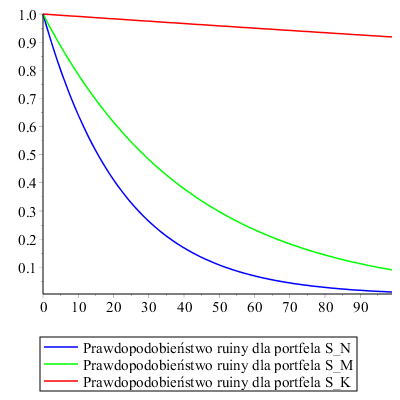
\includegraphics[scale=.7]{ruina}
\end{center}
\end{figure}
\end{document}